


\section{ANOVA}


\begin{frame}{Comparison of multiple means}{Introduction}

In previous lectures, we have (hopefully) developed a solid understanding of the main concepts associated with comparing the means of two groups;\bigskip

There are many cases, however, in which one may want to perform inference about differences of the means of multiple populations;\bigskip

\begin{columns}
  \column{.7\textwidth}
  We will develop the main concepts and ideas related with this kind of test by examining a simple example, related to a paper manufacturing operation.

  \column{.3\textwidth}
  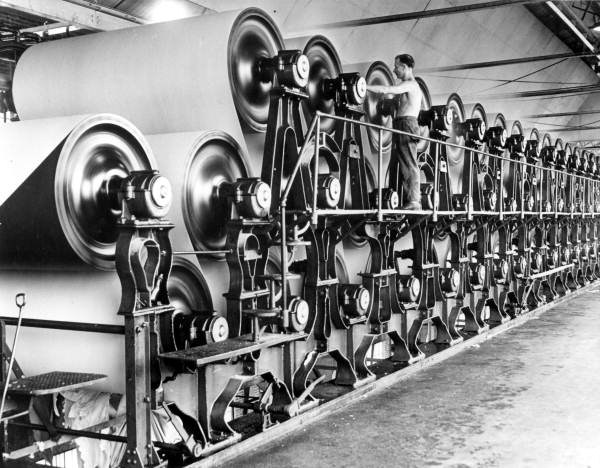
\includegraphics[width=\textwidth]{../img/papermill.jpg}
  \ppagenote{Paper Mill Image from \url{http://goo.gl/xYVW0M}}
\end{columns}
\end{frame}

\subsection{Motivating Example}
  \begin{frame}{Example: paper manufacturing}{Problem definition}
  Tensile strength (TS) is an important characteristic for certain types of paper for industrial use;
  \bigskip

  A reasonable conjecture is that this characteristic is influenced by the kind of wood fiber used in the manufacturing process.
  \bigskip

  The process engineer wants to investigate whether four different wood fibers result in papers with relevant differences of TS, using a pilot plant as his experimental unit.\footnote{Example adapted from Montgomery \& Runger (2010), Ch. 13.}
\end{frame}

\begin{frame}{Example: paper manufacturing}{Problem definition}

Suppose that the total budget allocated for the experiment allows only six production runs for each kind of wood fiber.
\bigskip

Under these specifications, the experiment has a single experimental \textit{factor} (\textit{wood fiber}) with $a = 4$ \textit{levels} (fiber types \textit{A}, \textit{B}, \textit{C} and \textit{D}) and $n = 6$ \textit{replicates} at each level.
\bigskip

The response variable will be the tensile strength of paper (measured, e.g., in kPa). The engineering team is interested in finding out whether any fiber type leads to an increase in the mean TS value of the paper.
\bigskip

The minimum difference of practical meaning is defined as $5 kPa$, and a reasonable upper estimate for the standard deviation of this process is $\hat{\sigma} = 6 kPa$. Desired error levels are defined as $\alpha = 0.1$ and $\beta = 0.2$.
\end{frame}


\begin{frame}[fragile]{Example: paper manufacturing}{Exploratory data analysis}
\begin{columns}
  \column{0.6\textwidth}
  It is always a good idea first to perform exploratory data analysis.\medskip

  As we are interested in the differences between the four wood types, we plot each of them as a boxplot and observe the differences.
  \column{0.4\textwidth}
  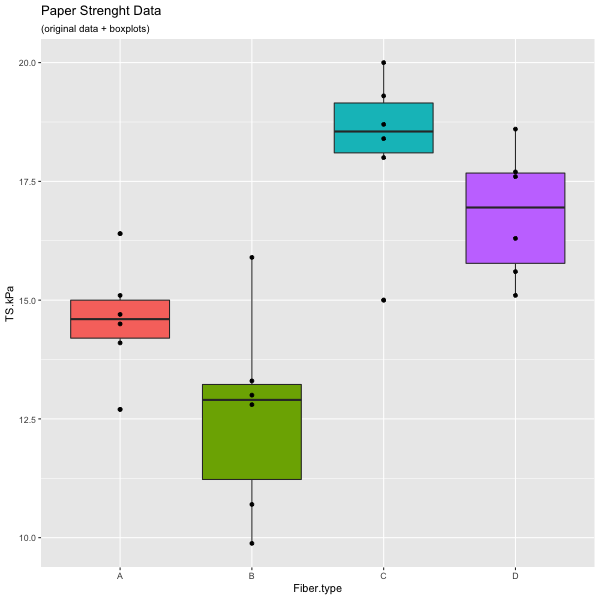
\includegraphics[width=1\textwidth]{../img/paperboxplot.png}
\end{columns}

{\tiny
\begin{verbatim}
> paper <- read.table(file   = "../data files/paper_strength.csv",
+                     header = TRUE, sep    = ",")

> library(ggplot2)
> ggplot(paper, aes(x = Fiber.type, y = TS.kPa, fill = Fiber.type)) +
+        geom_boxplot() + geom_point()
\end{verbatim}}
\end{frame}



%=====

\begin{frame}{Example: paper manufacturing}{Exploratory data analysis}
  \begin{columns}
    \column{.6\textwidth}
    The boxplot suggests the existence of differences among factor levels;
    \bigskip

    Besides, we can also observe a small variability in the spread of different levels; some suggestion of asymmetry in level \textit{B}; and a possible outlier in level \textit{C}.
    \bigskip

    These characteristics will need to be taken into account during the analysis.
    \column{.4\textwidth}
    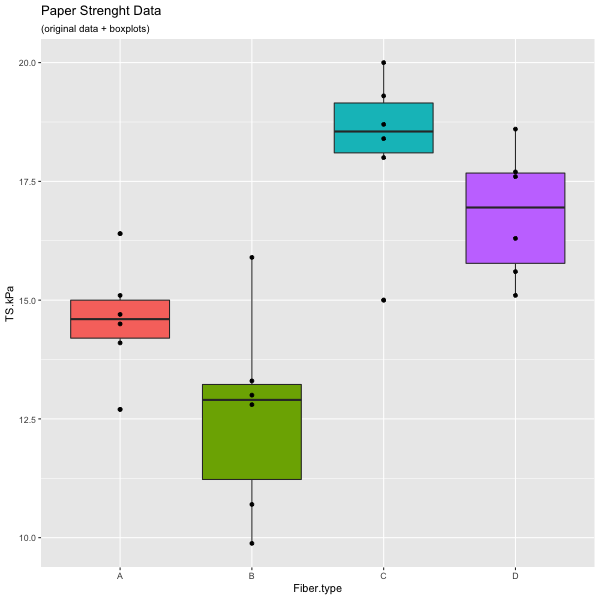
\includegraphics[width=1\textwidth]{../img/paperboxplot.png}
  \end{columns}
\end{frame}


% %=====
%

\begin{frame}
{Example: paper manufacturing}
{Statistical model}

This data can be described by a linear statistical model of the form:
\begin{equation*}
y_{ij} = \underbrace{\mu_i + \epsilon_{ij}}_{\mbox{\scriptsize Means model}} = \underbrace{\mu + \tau_i + \epsilon_{ij}}_{\mbox{\scriptsize Effects model}}\begin{cases}i=1,\ldots,a\\j=1,\ldots,n\end{cases}
\end{equation*}
where $\mu$ is the overall mean, $\tau_i$ represents the effect of the $i$-th level, and $\epsilon_{ij}$ is the residual (random error, or unmodeled variability);\bigskip

In the derivation of the statistical test for the existence of differences in the group means, we will employ the effects model, and initially consider a few assumptions about the residuals:
\begin{equation*}
y_{ij} = \mu + \tau_i + \epsilon_{ij}\begin{cases}i=1,\ldots,a\\j=1,\ldots,n\end{cases},\ \ \ \mbox{with }\epsilon_{ij} \overset{\mbox{\tiny i.i.d.}}{\sim}\mathcal{N}\left(0,\sigma^2\right)
\end{equation*}
\end{frame}


%=====

\begin{frame}
{Example: paper manufacturing}
{Statistical model}
If these assumptions are correct, the populations are expected to be distributed as:

\centering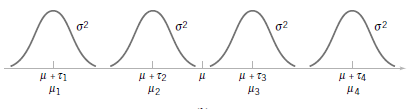
\includegraphics[width=0.7\textwidth]{../img/papermodels.png}
\ppagenote{Image from Montgomery\&Runger (2010), Ch. 13}

\vspace{-1em}
Since we are interested in testing our data for differences in the mean values of each population, the test hypotheses can be described as:

\begin{equation*}
\begin{cases}
H_0: \tau_i = 0,\ \ \forall i\in\left\{1,2,\ldots,a\right\}\\
H_1: \exists\ \tau_i \neq 0
\end{cases}\ \ \ \ \ \ \
\end{equation*}

If data collection is performed in random order, under constant experimental conditions, we have a \textit{completely randomized design}.
\end{frame}

\subsection{Fixed Effects Model}
\begin{frame}
{The Fixed Effects Model}{Definition}

This approach to modeling the mean effects of specific factor levels is known as the \textit{fixed effects model};
\bigskip

This approach is appropriate to testing hypotheses in situations when factor levels are arbitrarily defined by the experimenter;\bigskip

For these cases, the inference is made over the mean values for each level, and cannot be extended to similar levels that were not tested (e.g., other types of wood fiber);\bigskip

Other situations may require different kinds of modeling, such as \textit{random} or \textit{mixed effects models}, but these will not be explored here.
\end{frame}

%=====

\begin{frame}
{The Fixed Effects Model}
{Development}
As mentioned earlier, we will use the \textit{effects model} for describing the development of the statistical test:
\begin{equation*}
y_{ij} = \mu + \tau_i + \epsilon_{ij}\begin{cases}i=1,\ldots,a\\j=1,\ldots,n\end{cases}
\end{equation*}
\noindent where treatment effects are seen as deviations from the grand mean $\mu$.
\bigskip
By construction, we have that:
\begin{equation*}
\sum_{i=1}^{a}\tau_i = 0;
\end{equation*}
\end{frame}

%=====
%
\begin{frame}
{The Fixed Effects Model}
{Development}
The total variability of the data can be expressed by the \textit{total sum of squares}, which represents the sum of the squared deviations between each observation and the overall sample mean:
\begin{equation*}
SS_T = \sum_{i=1}^{a}{\sum_{j=1}^{n}{\left(y_{ij} - \bar{y}_{\bullet\bullet}\right)^2}}
\end{equation*}
With some relatively simple algebra, the $SS_T$ can be divided into two terms, representing the within-group and the between-group variability:
\begin{equation*}
SS_T = \sum_{i=1}^{a}{\sum_{j=1}^{n}{\left(y_{ij} - \bar{y}_{\bullet\bullet}\right)^2}}=\underbrace{n\sum_{i=1}^{a}{\left(\bar{y}_{i\bullet} - \bar{y}_{\bullet\bullet}\right)^2}}_{SS_{\mbox{\tiny\textit{Levels}}}} + \underbrace{\sum_{i=1}^{a}{\sum_{j=1}^{n}{\left(y_{ij}- \bar{y}_{i\bullet}\right)^2}}}_{SS_E}
\end{equation*}

\noindent where $\bullet$ indicates the summation over an index, and $\bar{\ \ }$ indicates an averaging operation.
\end{frame}
%
% %=====
%
\begin{frame}
{The Fixed Effects Model}
{Development}
Dividing the sums of squares by their respective number of degrees of freedom yields quantities known as \textit{mean squares}.
\bigskip

The relevant means squares for our test will be the \textit{levels mean square} and the \textit{residual mean square}:
\begin{equation*}
MS_E = \frac{SS_E}{a\left(n-1\right)}\ \ \ \ \ \ \ \ \ \ \ \ \ \ \ \ \ \ \ \
MS_{\mbox{\tiny\textit{Levels}}} = \frac{SS_{\mbox{\tiny\textit{Levels}}}}{a-1}
\end{equation*}
The expected values of these quantities are:
\begin{equation*}
E\left[MS_E\right] = \sigma^2\ \ \ \ \ \ \ \ \ \ \ \ \ \ E\left[MS_{\mbox{\tiny\textit{Levels}}}\right] = \sigma^2 + \frac{n\sum_{i=1}^{a}{\tau_i^2}}{a-1}
\end{equation*}

\end{frame}
%
% %=====
%
\begin{frame}
{The Fixed Effects Model}
{Development}
\begin{equation*}
E\left[MS_E\right] = \sigma^2\ \ \ \ \ \ \ \ \ \ \ \ \ \ E\left[MS_{\mbox{\tiny\textit{Levels}}}\right] = \sigma^2 + \frac{n\sum_{i=1}^{a}{\tau_i^2}}{a-1}
\end{equation*}

Notice that $MS_E$ is an unbiased estimator for the common variance of the residuals, while $MS_{\mbox{\tiny\textit{Levels}}}$ is biased by a term that is proportional to the squared values of the $\tau_i$ coefficients.
\bigskip

However, under $H_0$ we have that $\tau_i=0$ for all $i$, that is, $E\left[MS_{\mbox{\tiny\textit{Levels}}}\right] = E\left[MS_{E}\right] = \sigma^2$. \alert{\textit{But only if the null hypothesis is true}}.
\end{frame}
%
% %=====
%
\begin{frame}{The Fixed Effects Model}{Development}
It can be shown that, if $H_0$ is true, the statistic
\begin{equation*}
F_0 = \frac{MS_{\mbox{\tiny\textit{Levels}}}}{MS_E}
\end{equation*}
is distributed according to an $F$ distribution with $a-1$ degrees of freedom for the numerator and $a(n-1)$ for the denominator.  The usual notation is $F_{\left(a-1\right),a(n-1)}$
\bigskip

If $H_0$ is false, the expected value of $MS_{\mbox{\tiny\textit{Levels}}}$ is larger than that of $MS_E$, which results in larger values of $F_0$ and defines the critical region for our test:
\begin{block}{}
\centering Reject $H_0$ at the $\alpha$ significance level if\\$f_0>F_{1-\alpha;(a-1),a(n-1)}$
\end{block}
\end{frame}



%
% %=====
%
\subsection{Example Application}
\begin{frame}[fragile]
{Example: paper manufacturing}
{Computational analysis}

{\smaller
\begin{verbatim}
> my.model <- aov(TS.kPa ~ Fiber.type,
+              data = paper)
>
> summary.aov(my.model)

Df Sum Sq Mean Sq F value   Pr(>F)
Fiber.type   3 110.77   36.92   13.62 4.56e-05 ***
Residuals   20  54.24    2.71
---
Signif. codes:  0 '***' 0.001 '**' 0.01 '*' 0.05 '.' 0.1 ' ' 1
\end{verbatim}}

The \textit{ANOVA table} provides information on the sources of variation, together with their corresponding \textit{d.o.f.}, sums of squares and mean square values. The table also informs the values of the test statistic and the corresponding p-value of the test ($Pr(>F)$).
\bigskip

In this case, the p-value ($p = 4.56\times 10^{-5}$) suggests the rejection of the null hypothesis in favor of the alternative. But what does that mean?
\end{frame}

\begin{frame}
{Example: paper manufacturing}
{Computational analysis}
Recall the null and alternative hypotheses for the ANOVA:
\begin{equation*}
\begin{cases}
H_0: \tau_i = 0,\ \ \forall i\\
H_1: \exists\ \tau_i \neq 0
\end{cases}
\end{equation*}

The rejection of the null hypothesis leads to the conclusion that \textit{there is at least one level with an effect significantly different from zero}. But which one?
\bigskip

For this analysis to be complete, we still need to answer two questions:
\begin{itemize}
  \item Can we verify the assumptions of the test?
  \item Which means are different from which, and by how much?
\end{itemize}
\end{frame}


%
% %=====
%
\begin{frame}
{Assumptions}
{Model validation}
As mentioned earlier, the ANOVA model is based on three assumptions on the behavior of the residuals:
\begin{itemize}
  \item \textit{Independence};
  \item \textit{Homoscedasticity}, i.e., equality of variances across groups;
  \item \textit{Normality};
\end{itemize}
The residuals of the model can be easily obtained as:
\begin{equation*}
e_{ij} = y_{ij} - \hat{y}_{ij} = y_{ij} - \left(\hat{\mu} + \hat{\tau_i}\right) = y_{ij}-\bar{y}_{i\bullet}
\end{equation*}
\noindent or extracted directly from the fitted object in R using "my.model\$residuals"

\end{frame}
%
% %=====
%
\begin{frame}[fragile]
{Assumptions -- Model Validation}
{Normality Assumption}

\begin{columns}
  \column{.6\textwidth}
    The normality assumption can be tested using the Shapiro-Wilk test coupled with a normal QQ plot of the residuals.
    {\smaller
\begin{verbatim}
> shapiro.test(model$residuals)
Shapiro-Wilk normality test
data:  my.model$residuals
W = 0.9722, p-value = 0.7225

> library(car)
> qqPlot(my.model$residuals,
pch = 16, lwd = 3, cex = 2, las = 1)
\end{verbatim}}
    The ANOVA is relatively robust to moderate violations of normality, as long as the other assumptions are verified (or the sample size is large enough).
  \column{.4\textwidth}
    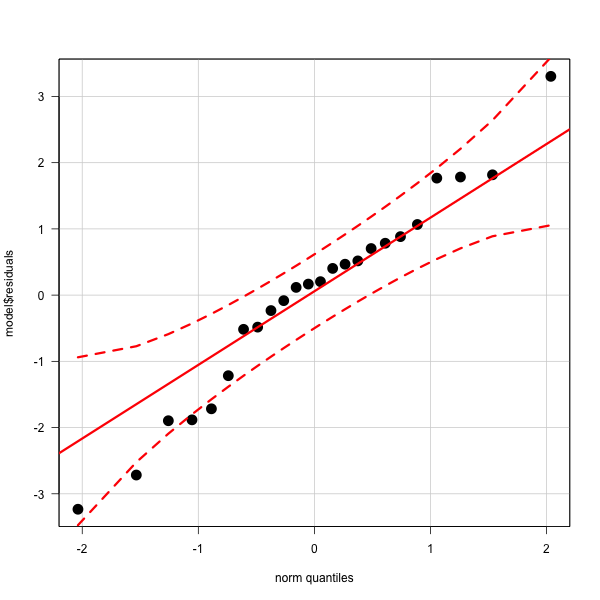
\includegraphics[width=1\textwidth]{../img/paperqq.png}
  \end{columns}
\end{frame}
%
% %=====
%
\begin{frame}[fragile]
{Assumptions -- Model Validation}
{Homoscedasticity Assumption (similar variances)}
\begin{columns}
  \column{.6\textwidth}
  The homoscedasticity assumption can be verified by the Fligner-Killeen test, together with plots of residuals by fitted values:

  {\smaller
\begin{verbatim}
> fligner.test(TS_kPa~Hardwood,
+              data = paper)
Fligner-Killeen test of homogeneity of
variances
data:  data:  TS.kPa by Fiber.type
Fligner-Killeen:
med chi-squared = 1.0622, df = 3,
p-value = 0.7862
> plot(x = my.model$fitted.values,
+      y = my.model$residuals)

\end{verbatim}}

  \column{.4\textwidth}
  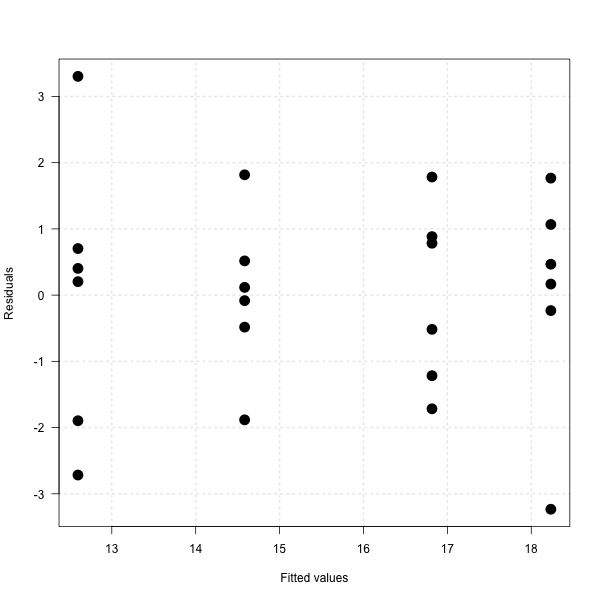
\includegraphics[width=\textwidth]{../img/papervar.png}
\end{columns}
ANOVA is relatively robust to modest violations of homoscedasticity, as far as the sample is \textit{balanced}.

\end{frame}
%
% %=====
%
\begin{frame}[fragile]
{Assumptions -- Model Validation}
{Independence Assumption}
As usual, the independence assumption should be guaranteed (to the best of the experimenter's knowledge) on the design phase, as well as on the analysis. This includes avoiding pseudoreplication and ordering effects, among others.
\bigskip

To test for serial correlations, we can use the Durbin-Watson test, but that only really makes sense if the data is presented to the DW test ordered by an unmodelled and possibly influential variable (such as by order of data collection).\bigskip
%\vhalf
%\begin{rcode}
%> durbinWatsonTest(model)
% lag Autocorrelation D-W Statistic p-value
%   1    -0.008996302      1.872801   0.868
% Alternative hypothesis: rho != 0
%
%> plot(x    = seq_along(model$residuals),
%+      y    = model$residuals,
%+      type = "l", ...)
%> points(x    = seq_along(model$residuals),
%+        y    = model$residuals,
%+        type = "p",
%+        col  = as.numeric(paper[,1]), ...)
%\end{rcode}

The ANOVA can be quite sensitive to violations of independence. Randomization and attention to possibly influential factors can help avoiding violations of this assumption.
%\begin{tikzpicture}[remember picture,overlay]
%\node[anchor=north east,yshift=-78pt,xshift=0pt] at (current page.north east) {\includegraphics[width=.43\textwidth]{../Images/paperind.png}};
%\end{tikzpicture}
\end{frame}
%
% %=====
%

\subsection{Comparisons Post ANOVA}

\begin{frame}
{Multiple comparisons}
{The need for multiple comparisons}

If the ANOVA assumptions are verified (i.e., if we have solid grounds for trusting the result of the test), we usually need to determine \textit{which} levels of the factor are significantly different\footnote[1]{\tiny Of course this is only necessary if we rejected $H_0$ in the original test. For more on how to proceed with nonsignificant results, see Ellis(2010).};
\bigskip

Whenever possible, the planning of which comparisons will be after an analysis of variance procedure should be defined \textit{a priori}. Post-hoc definition of hypotheses (a.k.a.  HARKing\footnote[2]{\tiny\textbf{H}ypothesizing \textbf{A}fter the \textbf{R}esults are \textbf{K}nown. See Kerr(1998).}) are a common entry point for researcher biases into the analysis, and should be dealt with very carefully.
\end{frame}
%
% %=====
%
\begin{frame}
{Multiple comparisons}
{Types of comparisons}
The planning of multiple comparisons must be guided by the technical question underlying the experiment.\bigskip

Whenever possible, the researcher should opt to perform the smallest number of comparisons needed to adequately answer his or her question. This will require the smallest sample size, or result in the largest power for a given experimental setup.\bigskip

Usual questions involve (but are not limited to):

\begin{itemize}
  \item \textit{How does one level compare to the others?}
  \item \textit{How does each level compare to the grand mean?}
  \item \textit{How do the levels compare to each other (all vs. all)?}
\end{itemize}
\end{frame}
%
% %=====
%
\begin{frame}
{Multiple comparisons}
{MHT considerations}
The multiple comparisons performed after an ANOVA are essentially composed of a series of t-tests for the difference between two population means, with some slight modifications;
\bigskip

If the assumptions of the ANOVA are verified, we already have some information about the data: we know, for instance, that the groups are homoscedastic, and that their common variance is estimated by $MS_E$, with $a(n-1)$ degrees of freedom;
\bigskip

We also know that, if we are going to perform multiple tests on the same data set, that the probability of a type-I error on each test is $\alpha$. If we want to to keep our overall error rate controlled at a given level, we will need to correct the $\alpha$ value used for each test.%
%\footnote{\tiny This value is the one that should be used in sample size calculations. There are ways to estimate sample sizes for the omnibus ANOVA, but we'll (almost) always want to pinpoint the differences afterwards.}.
\end{frame}
%
% %=====
%
\begin{frame}
{Multiple comparisons}
{MHT corrections}

There are a number of ways of adjusting the $\alpha$ value of the pairwise comparisons in order to maintain the \textit{familywise error rate} (FWER) at a controlled level\footnote[3]{The methods presented here work well for a relatively small number of comparisons. For more on MHT, see Schaffer(1995)'s discussion on controlling the False Discovery Rate.}.\bigskip

Two of the most common (and most conservative) are the Bonferroni and the \v{S}id\'ak corrections. Assuming $K$ planned comparisons, the Bonferroni method tests each individual hypothesis with:

\begin{equation*}
\alpha_{adj}=\frac{\alpha_{\mbox{\scriptsize \textit{family}}}}{K}
\end{equation*}

\noindent while the \v{S}id\'ak correction uses:

\begin{equation*}
\alpha_{adj}=1 - \left(1-\alpha_{\mbox{\scriptsize \textit{family}}}\right)^{1/K}
\end{equation*}
\end{frame}
%
% %=====
%
\begin{frame}
{Multiple comparisons}
{All vs. all}
Pairwise comparisons of the \textit{all vs. all} type appear whenever we are simply interested in detecting which levels are significantly different from which, without any prior information or special interest in one specific level or ordering.\bigskip

In these cases, the number of comparisons is $K=a(a-1)/2$, where $a$ is the number of levels.\bigskip

The sample size calculations for this case can follow the same equations used for the t test for two independent samples, but with the $\alpha$ value corrected for multiple hypotheses and the number of degrees of freedom of the reference distribution equal to those of the residual term in the ANOVA, i.e., $a(n-1)$.
\end{frame}
%
% %=====
%
\begin{frame}
{Multiple comparisons}
{All vs. all}
For performing \textit{all vs. all} multiple comparisons, a common alternative is to use Tukey's \textit{Honest Significant Difference} (HSD) approach. This method is generally chosen because it provides a slightly higher power when compared to the Bonferroni correction\footnote[4]{\tiny The difference is due to Tukey's approach using a modified value for the $t_{\beta}$ term in the power calculations. See Mathews (2011) and Montgomery (2010) for details.}.\bigskip

A simple approach is to calculate the sample size using Bonferroni-corrected $\alpha$-values (for simplicity), and performing the tests using Tukey's HSD corrections (for increased power):

\begin{equation*}
n \approxeq 2\left(\frac{\left(t_{(\alpha_{adj}/2)}+t_{\beta}\right)\hat{\sigma}}{\delta^*}\right)^2
\end{equation*}
\noindent with $a(n-1)$ degrees of freedom for the $t$ variables.
\end{frame}
%
% %=====
%
\begin{frame}[fragile]
{Multiple comparisons}
{All vs. all}
%Suppose that was the case for our wood fiber example:

\begin{columns}
  \column{0.6\textwidth}
{\smaller
\begin{verbatim}
> library(multcomp)
> mc1    <- glht(my.model, linfct = mcp(Fiber.type = "Tukey"))
> mc1_CI <- confint(mc1, level = 0.95)

Simultaneous Confidence Intervals
Multiple Comparisons of Means:
95% family-wise confidence level

Linear Hypotheses:
           Estimate lwr     upr
B - A == 0 -1.9867  -4.6478  0.6745
C - A == 0  3.6500   0.9889  6.3111
D - A == 0  2.2333  -0.4278  4.8945
C - B == 0  5.6367   2.9755  8.2978
D - B == 0  4.2200   1.5589  6.8811
D - C == 0 -1.4167  -4.0778  1.2445
> plot(mc1_CI)
\end{verbatim}}
\column{.4\textwidth}
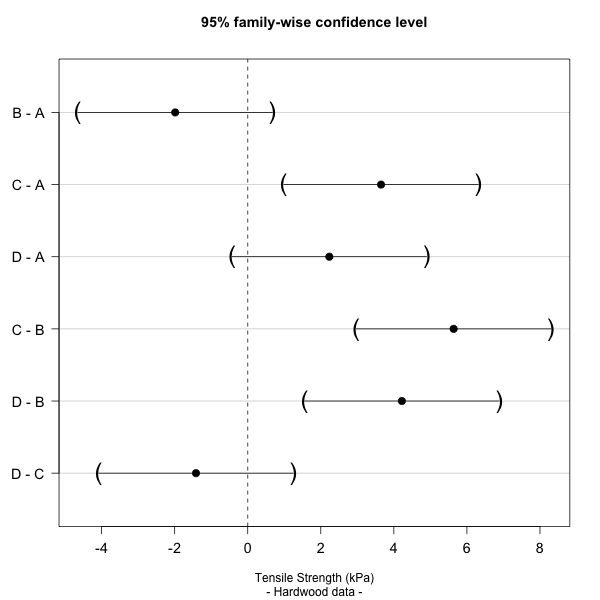
\includegraphics[width=1\textwidth]{../img/papertukey.png}
\end{columns}
\end{frame}
%
% %=====
%
\begin{frame}
{Multiple comparisons}
{All vs. one}
Pairwise comparisons of the \textit{all vs. one} type usually emerge in the context of comparing levels against a control:

\begin{itemize}
  \item Comparison of a proposed approach vs. existing ones;
  \item Comparison of different approaches vs. a standard one (or a placebo-like group);
\end{itemize}
In these cases, the number of comparisons is $K = a-1$, where $a$ is the number of levels. Each test can again be performed (at least in principle) using the $t_0$ test statistic:

\begin{equation*}
t^i_0 = \frac{\bar{y}_i - \bar{y}_0}{\hat{\sigma}\sqrt{\left(\frac{1}{n_i}+\frac{1}{n_0}\right)}}
\end{equation*}
\end{frame}
%
% %=====
%
\begin{frame}
{Multiple comparisons}
{All vs. one}
There are two main approaches to calculating sample size for \textit{all vs. one} comparisons:

\begin{itemize}
  \item Balanced design;
  \item Optimal allocation of units.
\end{itemize}

With a balanced design (that is, all levels have the same number of observations), the calculation of $n$ follows the same approach as the \textit{all vs. all} comparisons, but correcting $\alpha$ for only $a-1$ comparisons.\bigskip

For the optimal allocation of units, an unbalanced design is used.
\end{frame}
%
% %=====
%
\begin{frame}
{Multiple comparisons}
{All vs. one - optimal allocation}

As several levels will be compared against the single control group, the relative importance of the latter is greater and therefore it should have a larger sample size.
\bigskip

To maximize the power of this multiple comparisons procedure, the sample size of the control group should be:
\begin{equation*}
n_0 = n_i\sqrt{K}
\end{equation*}

\noindent where $n_i$ is the common sample size for the non-control levels:
\begin{equation*}
n_i \approxeq \left(1 + \frac{1}{\sqrt{K}}\right)\left(\frac{(t_{(\alpha_{adj}/2)}+t_{\beta})\hat{\sigma}}{\delta^*}\right)^2
\end{equation*}
\footnote{A good free software for doing sample size calculations and power analysis in nontrivial contexts such as this one is G*Power 3, \url{http://www.gpower.hhu.de/} . It is also relatively simple to implement these calculations in R.}
\end{frame}
%
% %=====
%
\begin{frame}
{Multiple comparisons}
{All vs. one - \textbf{Dunnett's test}}
As in the case of \textit{all vs. all} comparisons, there is a test that is usually employed for its superior sensitivity: Dunnett's test.\bigskip

The control group sample size $n_0$ calculated assuming that Bonferroni-corrected t-tests will be used is slightly overestimated in relation to the required $n_0$ for Dunnett's test, but in practice the differences are small enough not to matter;
\end{frame}
%
% %=====
%
\begin{frame}[fragile]
{Multiple comparisons}
{All vs. one}
Assuming that in our example the \textit{B} level is the standard one, against which the other ones are to be compared:

\begin{columns}
  \column{.6\textwidth}
  {\tiny
\begin{verbatim}
> paper$Fiber.type <- relevel(paper$Fiber.type,
                              ref = "B")
> model2           <- aov(TS.kPa ~ Fiber.type,
                          data = paper)
> mc2              <- glht(model2,
                       linfct = mcp(Fiber.type = "Dunnett"))
> mc2_CI           <- confint(mc2, level = 0.95)

Simultaneous Confidence Intervals
Multiple Comparisons of Means: Dunnett Contrasts
95% family-wise confidence level
Linear Hypotheses:
Estimate lwr     upr
A - B == 0  1.9867  -0.4275  4.4008
C - B == 0  5.6367   3.2225  8.0508
D - B == 0  4.2200   1.8058  6.6342

> plot(mc2_CI)
\end{verbatim}}
  \column{.4\textwidth}
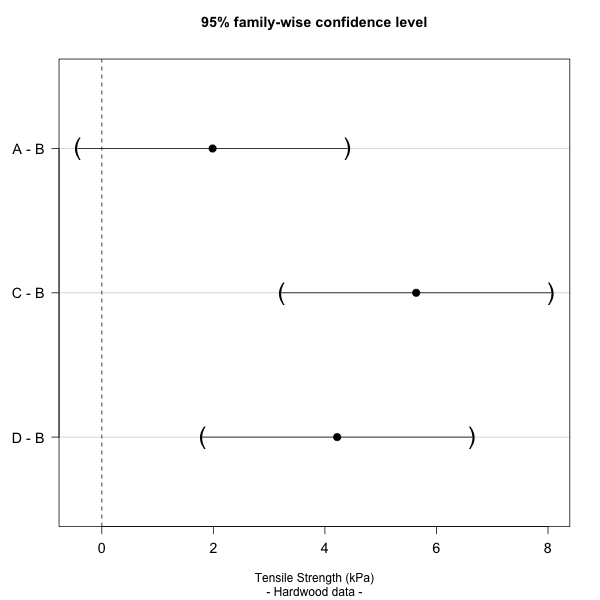
\includegraphics[width=1\textwidth]{../img/paperdunnett.png}
\end{columns}
\end{frame}
%
% %=====
%
\begin{frame}
{Multiple comparisons}
{Some final considerations}
The kind of comparisons that are to be performed after an ANOVA should be planned in advance, as it influences your data collection and sample size calculations. There are of course sample size formulas for the pure ANOVA, but these are usually of limited use since researchers frequently want to know where the detected differences lie.
\bigskip

There are a myriad of approaches for post-ANOVA multiple comparisons\footnote[5]{\tiny Check Hothorn \textit{et al.} (2008) for an idea on how varied this can get.}, but in general the formulas for sample size calculation will follow the ideas outlined above: correct the $\alpha$ value to account for type-I error inflation and calculate $n$ based on formulas for two-sample $t$ tests.
\end{frame}
%










%%%%%%%%%%%%%%%%%%%%%%%%% Sample Sizes %%%%%%%%%%%%%%%%%%%%%

% %=====
%
% \begin{ftst}
% {More on sample sizes}
% {Sample size formulas for ANOVA}
% If one is interested in calculating the required sample size for the ANOVA procedure (without worrying about the eventual post-hoc testing), the formulas are almost as simple as those used for the t tests.
% \vone
% Essentially, the power/sample size calculations for the ANOVA boil down to the equality:
%
% \beqs
% F_{(1-\alpha)} = F_{\beta;\phi}
% \eqs
%
% with both $F$ distributions having $(a-1)$ degrees of freedom in the numerator and $a(n-1)$ in the denominator. The noncentrality parameter $\phi$ is given by:
%
% \beqs
% \phi = \frac{n\sum\limits_{i=1}^{a}\tau_i^2}{\hat{\sigma}^2}
% \eqs
% \end{ftst}
%
% %=====
%
% \begin{ftst}
% {More on sample sizes}
% {Sample size formulas for ANOVA}
% To ilustrate the sample size calculation procedure, imagine an experimental design with $a = 4,\ \alpha = 0.05,\ \hat{\sigma} = 7$, and suppose that the researcher wants to be able to detect whether any two means present differences of magnitude $\delta^* = 12$ with power $(1-\beta)=0.8$.
% \vone
% Under these conditions, two scenarios tend to be of interest: the first is if we have two levels biased symmetrically about the grand mean, and all the others equal to zero:
%
% $$ \tau = \left\{-\frac{\delta^*}{2}, \frac{\delta^*}{2}, 0, 0\right\}$$
%
% \noindent and the second is if we have one level biased in relation to all others:
%
% $$ \tau = \left\{-\frac{(a-1)\delta^*}{a}, \frac{\delta^*}{a}, \frac{\delta^*}{a}, \frac{\delta^*}{a}\right\}$$
%
% \end{ftst}
%
% %=====
%
% \begin{ftst}
% {More on sample sizes}
% {Sample size formulas for ANOVA}
% For the first case we have a noncentrality parameter of:
%
% $$\phi = \frac{4\left(6^2+6^2+0+0\right)}{7^2} = 5.88$$
%
% Which allows us to calculate the required sample size by iterating on $n$ until:
%
% $$F_{(1-\alpha)} \leq F_{\beta;\phi}$$
%
% \end{ftst}
%
% %=====
%
% \begin{ftstf}
% {More on sample sizes}
% {Sample size formulas for ANOVA}
% Doing it manually:
% \begin{verbatim}
% > a       <- 4
% > alpha   <- 0.05
% > sigma   <- 7
% > delta   <- 12
% > beta    <- 0.2
% >
% > tau <- c(-delta/2, delta/2, rep(0, a - 2)) # define tau vector
% > n   <- 2
% > while (qf(1 - alpha, a - 1, a*(n - 1)) >
% +        qf(beta, a - 1, a*(n - 1), n*sum(tau^2)/sigma^2)) n <- n + 1
% > print(n)
% [1] 9
% \end{verbatim}
% \vhalf
% Using \verb|power.anova.test()|:
% \begin{verbatim}
% > vartau <- var(tau)
% > power.anova.test(groups = 4, between.var = vartau,
% +                  within.var = sigma^2, sig.level = alpha,
% +                  power = 1 - beta)$n
% [1] 8.463358
% \end{verbatim}
% \end{ftstf}
%
% \begin{ftstf}
% {More on sample sizes}
% {Sample size formulas for ANOVA}
% The second case (one level biased in relation to all others) is also quite easy to calculate manually, but lets keep it simple:
%
% \begin{verbatim}
% > tau <- c(-delta*(a - 1)/a, rep(delta/a, a - 1))
% > vartau <- var(tau)
% > power.anova.test(groups = 4, between.var = vartau,
% +                  within.var = sigma^2, sig.level = alpha,
% +                  power = 1 - beta)$n
% [1] 6.018937
% \end{verbatim}
% \vone
% It is important to remember that these are the sample sizes required for the ANOVA only - any multiple comparisons procedure executed afterwards to pinpoint the significant differences will have smaller power for same-sized effects (unless more observations are added). This is one reason why it is common to design experiments calculating the sample sizes based on the multiple comparisons procedure, instead of using the ANOVA formulas.
% \end{ftstf}
